\documentclass{article}

\usepackage{amsfonts}
\usepackage{amssymb}
\usepackage{amsmath}
\usepackage{multicol}
\usepackage{xcolor}

\usepackage{tikz}
\usetikzlibrary{angles, quotes}

\begin{document}

\section{Vettori}

\subsection{Notazione}

$\vec{a} \in \mathbb{R}^n$

$$
\vec{a} = (a_1, a_2, \dots, a_n) : a_j \in \mathbb{R}^n
$$

\subsection{Definizioni}

\begin{description}
\item[Quantità scalari] sono le quantità definite da un numero (un vettore unidimensionale) e un'unità di misura (esempio: temperatura)
\item[Quantità vettoriali] definite da un vettore $\vec{a} \in \mathbb{R}^n : n > 1$ e un unità di misura (esempio: distanza)
\item[Quantità tensoriali] ??
\end{description}

\subsection{Rappresentazione grafica}

Un vettore è rappresentato da una freccia, che ha:

\begin{itemize}
\item Una direzione
\item Un verso
\item Modulo (un valore assoluto ed è la lunghezza della suddetta freccia)
\end{itemize}

\noindent
Dato un $\vec{a}$, il suo inverso è un vettore che ha uguale modulo ma verso opposto.

\subsection{Somma}

Regola del parallelogramma:

\begin{multicols}{2}
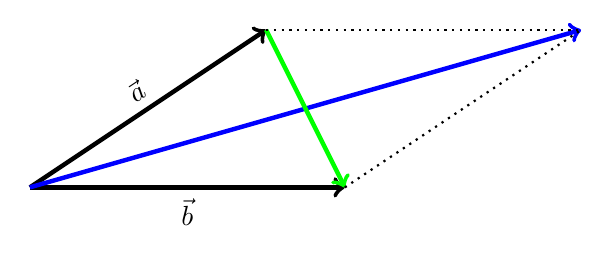
\begin{tikzpicture}
\coordinate (O) at (0,0);

\draw[ultra thick,black,->] (O) -- (3,2) coordinate(a) node[midway,above,sloped]{$\vec{a}$};
\draw[ultra thick,black,->] (O) -- (4,0) coordinate(b) node[midway,below,sloped]{$\vec{b}$};

\draw[ultra thick,blue,->] (O) -- (7,2) coordinate(c);
\draw[ultra thick,green,->] (a) -- (b);

\draw[thick,dotted,black] (a) -- (c);
\draw[thick,dotted,black] (b) -- (c);
\end{tikzpicture}

\begin{itemize}
\item \textcolor{blue}{blu $= \vec{a} + \vec{b}$}
\item \textcolor{green}{verde $= \vec{a} - \vec{b}$}
\end{itemize}
\end{multicols}

\subsection{Prodotto per scalare}

Dati $\lambda \in \mathbb{R}$ e $\vec{a} \in \mathbb{R}^n$, $\vec{b} = \lambda \vec{a} \in \mathbb{R}^n$ è un vettore con stessa direzione di $\vec{a}$ se:

\begin{itemize}
\item Se $\lambda > 0$, stesso verso
\item Se $\lambda < 0$, verso opposto
\end{itemize}

\noindent
Il modulo di $\vec{b}$ è uguale a $|\lambda|$ volte quello di $\vec{a}$

\subsection{Prodotto scalare}

Un operazione che prende due vettori e restituisce un numero.

\begin{center}
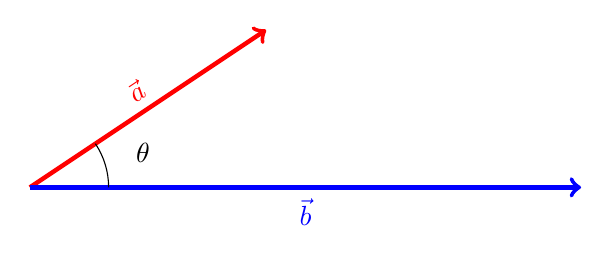
\begin{tikzpicture}
\coordinate (O) at (0,0);

\draw[ultra thick,red,->] (O) -- (3,2) coordinate(a) node[midway,above,sloped]{$\vec{a}$};
\draw[ultra thick,blue,->] (O) -- (7,0) coordinate(b) node[midway,below,sloped]{$\vec{b}$};

\pic[draw=black, "$\theta$", angle eccentricity=1.5, angle radius=10mm]{angle=b--O--a};
\end{tikzpicture}
\end{center}

$$
\vec{a} * \vec{b} = |\vec{a}| * |\vec{b}| * \cos{\theta}
$$

\noindent
Dove $|\vec{a}|$ è il modulo di $|\vec{a}|$ (similmente per $\vec{b}$) e $\theta$ è l'angolo compreso tra $\vec{a}$ e $\vec{b}$.

\subsubsection{Proprietà}

\begin{itemize}
\item Commutativa: $\vec{a} * \vec{b} = \vec{b} * \vec{a}$
\item Distributiva: $\vec{a} * (\vec{b}+\vec{c}) = \vec{a}*\vec{b} + \vec{a}*\vec{c}$
\item $\forall \lambda \in \mathbb{R} : \lambda (\vec{a} * \vec{b}) = (\lambda\vec{a}) * \vec{b} = \vec{a} * (\lambda\vec{b})$
\end{itemize}

\subsection{Componente}

Dato $\vec{a} \in \mathbb{R}^n$ e vettore di modulo 1 (vettore unitario)  $\vec{u} \in \mathbb{R}^n$, definiamo la componente di $\vec{a}$ lungo $\vec{u}$ il numero:

$$
\vec{a} * \vec{u} = |\vec{a}| * |\vec{u}| * \cos{\theta} = |\vec{a}| * \cos{\theta}
$$

\subsubsection{Versore}

Chiamiamo versori i vettori di modulo 1, e li indichiamo con $\hat{u}$.

\subsubsection{Vettore componente}

Dati $\vec{a}, \hat{u}$, definiamo il vettore componente $\vec{a}_u$ come il vettore lungo $\hat{u}$ con modulo $|\vec{a} * \hat{u}|$.

$$
\vec{a}_u = a_{\hat{u}} * \hat{u}
$$

\noindent
Il modulo di un vettore (o norma) è legato al prodotto scalare da $|a^2| = \vec{a} * \vec{a}$, infatti $\vec{a} * \vec{a} = |a| * |a| * \cos{\theta}$.

\subsection{Prodotto vettoriale}

Un operazione che prende 2 vettori e restituisce un vettore in $\mathbb{R}^3$.

$$
\vec{a} \wedge \vec{b} \text{ ("a vettor b")}
$$

\noindent
$\vec{a} \wedge \vec{b}$ è definito come il vettore che vive lungo la direzione ortogonale al piano individuato da $\vec{a}$ e $\vec{b}$, che ha modulo $|\vec{a}|*|\vec{b}|*\sin{\theta}$ e un verso determinato dalla "regola della mano destra".

\begin{center}
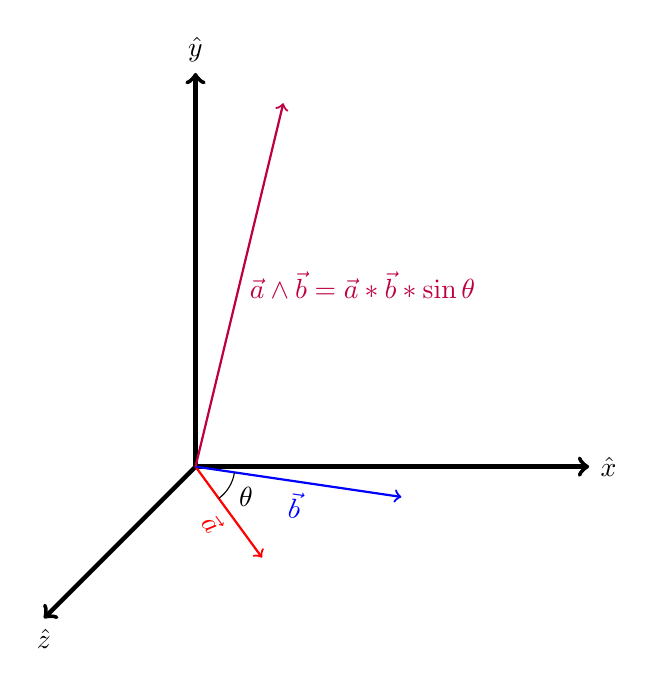
\begin{tikzpicture}
\coordinate (O) at (0,0,0);

\draw[ultra thick,black,->] (O) -- (5,0,0) coordinate(x) node[right]{$\hat{x}$};
\draw[ultra thick,black,->] (O) -- (0,5,0) coordinate(y) node[above]{$\hat{y}$};
\draw[ultra thick,black,->] (O) -- (0,0,5) coordinate(z) node[below]{$\hat{z}$};

\draw[thick,red,->] (O) -- (2,0,3) coordinate(a) node[midway,below,sloped]{$\vec{a}$};
\draw[thick,blue,->] (O) -- (3,0,1) coordinate(b) node[midway,below,sloped]{$\vec{b}$};
\draw[thick,purple,->] (O) -- (1.5,5,1) coordinate(c) node[midway,right]{$\vec{a} \wedge \vec{b} = \vec{a} * \vec{b} * \sin{\theta}$};

\pic[draw=black, "$\theta$", angle eccentricity=1.5, angle radius=5mm]{angle=a--O--b};
\end{tikzpicture}
\end{center}

\subsubsection{Proprietà}

\begin{itemize}
\item Distributiva: $(\vec{a} * \vec{b}) \wedge \vec{c} = \vec{a} \wedge \vec{c} + \vec{b} \wedge \vec{c}$
\item Non vale la proprietà associativa: $(\vec{a} \wedge \vec{b}) \wedge \vec{c} \neq \vec{a} \wedge (\vec{b} \wedge \vec{c})$
\end{itemize}

\subsection{Vettori e coordinate}

Possiamo passare ad una trattazione algebrica dei vettori introducendo un sistema di riferimento.
Questo significa introdurre un insieme di vettori privilegiato ed esprimere ogni altro vettore in termini delle componenti corrispondente.

\noindent
In una dimensione, un sistema di riferimento è dato da un singolo versore $\hat{u}$:

\begin{center}
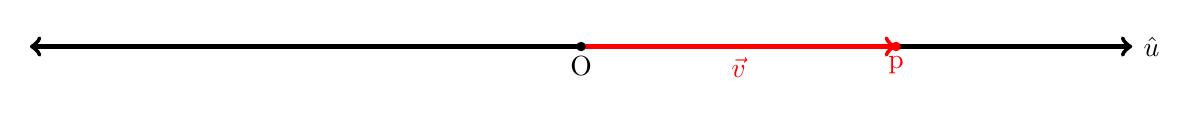
\begin{tikzpicture}
\coordinate (O) at (0,0);
\coordinate (p) at (4,0);

\draw[ultra thick,black,<->] (-7,0) -- (7,0) coordinate(u) node[right]{$\hat{u}$};
\draw[ultra thick,red,->] (O) -- (p) coordinate(v) node[midway,below]{$\vec{v}$};

\filldraw[black] (O) circle(1.5pt) node[below]{O};
\filldraw[red] (p) circle(1.5pt) node[below]{p};
\end{tikzpicture}

$$
\begin{matrix}
\vec{v} = v_{\hat{u}} * \hat{u} \\
|\vec{v}| = \vec{v} * \hat{u} = |\vec{v}_{\hat{u}}|
\end{matrix}
$$
\end{center}

\noindent
In due dimensioni, un sistema di riferimento è dato da due versori ortogonali:

\begin{center}
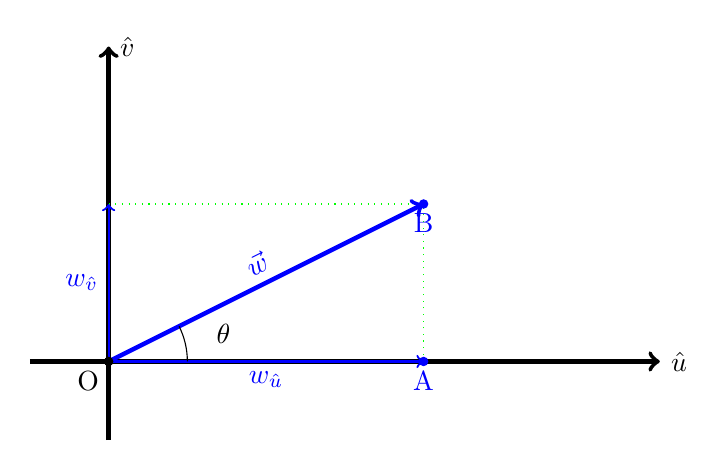
\begin{tikzpicture}
\coordinate (O) at (0,0);
\coordinate (A) at (4,0);
\coordinate (B) at (4,2);
\coordinate (C) at (0,2);

\draw[ultra thick,black,->] (-1,0) -- (7,0) coordinate(u) node[right]{$\hat{u}$};
\draw[ultra thick,black,->] (0,-1) -- (0,4) coordinate(v) node[right]{$\hat{v}$};

\draw[dotted,green] (A) -- (B);
\draw[dotted,green] (C) -- (B);

\draw[thick,blue,->] (O) -- (A) coordinate(w_u) node[midway,below]{$w_{\hat{u}}$};
\draw[thick,blue,->] (O) -- (C) coordinate(w_v) node[midway,left]{$w_{\hat{v}}$};
\draw[ultra thick,blue,->] (O) -- (B) coordinate(w) node[midway,above,sloped]{$\vec{w}$};

\pic[draw=black, "$\theta$", angle eccentricity=1.5, angle radius=10mm]{angle=w_u--O--w};

\filldraw[black] (O) circle(1.5pt) node[anchor=north east]{O};
\filldraw[blue] (A) circle(1.5pt) node[below]{A};
\filldraw[blue] (B) circle(1.5pt) node[below]{B};
\end{tikzpicture}

$$
\vec{w} = w_{\hat{u}} \hat{u} + w_{\hat{v}} \hat{v} \to (w_{\hat{u}}, w_{\hat{v}}) \in \mathbb{R}^2
$$
\end{center}

\noindent
In tre dimensioni, un sistema di riferimento è determinato da tre versori ortogonali (di solito i versori sono indicati come $\hat{x}, \hat{y}, \hat{z}$ oppure come $\hat{i}, \hat{j}, \hat{k}$):

\begin{center}
\begin{tikzpicture}
\coordinate (O) at (0,0,0);

\draw[ultra thick,black,->] (O) -- (7,0,0) coordinate(j) node[right]{$\hat{j}$};
\draw[ultra thick,black,->] (O) -- (0,4,0) coordinate(k) node[above]{$\hat{k}$};
\draw[ultra thick,black,->] (O) -- (0,0,4) coordinate(i) node[below]{$\hat{i}$};
\end{tikzpicture}
\end{center}

\noindent
Siccome i versori sono ortogonali: $\hat{i} \wedge \hat{j} = \hat{k}, \hat{j} \wedge \hat{i} = -\hat{k}$

\subsection{Operazioni tra vettori in coordinate}

Le coordinate sono le componenti di un vettore rispetto ai versori (o "assi") del sistema di riferimento.

\begin{description}
\item[Somma] $\vec{a} = (a_x, a_y, a_z), \vec{b} = (b_x, b_y, b_z)$

$$
\vec{a} + \vec{b} = (a_x+b_x, a_y+b_y, a_z+b_z)
$$

\item[Prodotto per scalare] $\lambda \in \mathbb{R}, \vec{a} \in \mathbb{R}^3, \vec{a} = (a_x, a_y, a_z)$

$$
\lambda \vec{a} = (\lambda a_x, \lambda a_y, \lambda a_z)
$$

\item[Prodotto scalare] $\vec{a} = a_i \hat{i} + a_j \hat{j} + a_k \hat{k}, \vec{b} = b_i \hat{i} + b_j \hat{j} + b_k \hat{k}$

$$
\begin{matrix}
\vec{a} * \vec{b} = a_ib_i + a_jb_j + a_kb_k \\
\vec{a} * \vec{b} = |\vec{a}| |\vec{b}| \cos{\theta} \\
\theta = \arccos{[\frac{a_ib_i + a_jb_j + a_kb_k}{|\vec{a}||\vec{b}|}]}
\end{matrix}
$$

\item[Prodotto vettoriale] $\vec{a} = a_i \hat{i} + a_j \hat{j} + a_k \hat{k}, \vec{b} = b_i \hat{i} + b_j \hat{j} + b_k \hat{k}$

$$
\vec{a} \wedge \vec{b} = (a_jb_k - a_kb_j, a_kb_i - a_ib_k, a_ib_j - a_jb_i)
$$
\end{description}

\subsection{Regola mnemonica del determinante}

Le componenti di $\vec{a} \wedge \vec{b}$ si ottengono calcolando il determinante di:

$$
\det{
\begin{pmatrix}
\hat{i} & \hat{j} & \hat{k} \\
a_i & a_j & a_k \\
b_i & b_j & b_k
\end{pmatrix}
} = \hat{i} (a_jb_k - a_kb_j) - \hat{j} (a_ib_k - a_kb_i) + \hat{k} (a_ib_j - a_jb_i)
$$

\end{document}
